\documentclass[a4paper]{article}
\usepackage[T1]{fontenc}			% \chapter package
\usepackage[english]{babel}
\usepackage[english]{isodate}  		% date format
\usepackage{graphicx}				% manage images
\usepackage{amsfonts}
\usepackage{booktabs}				% high quality tables
\usepackage{amsmath}				% math package
\usepackage{amssymb}				% another math package (e.g. \nexists)
\usepackage{bm}                     % bold math symbols
\usepackage{mathtools}				% emphasize equations
\usepackage{stmaryrd} 				% '\llbracket' and '\rrbracket'
\usepackage{amsthm}					% better theorems
\usepackage{enumitem}				% manage list
\usepackage{pifont}					% nice itemize
\usepackage{cancel}					% cancel math equations
\usepackage{caption}				% custom caption
\usepackage[]{mdframed}				% box text
\usepackage{multirow}				% more lines in a table
\usepackage{textcomp, gensymb}		% degree symbol
\usepackage[x11names]{xcolor}		% RGB color
\usepackage[many]{tcolorbox}		% colorful box
\usepackage{multicol}				% more rows in a table (used for the lists)
\usepackage{listings}
\usepackage{url}
\usepackage{qrcode}
\usepackage{fontawesome5}
\usepackage{ragged2e}
\usepackage{cite}                   % references
\usepackage{imakeidx}               % index
\makeindex[program=makeindex, columns=1,
           title=Index, 
           intoc,
           options={-s index-style.ist}]

\usepackage{fancyhdr}


\definecolor{codegreen}{rgb}{0,0.6,0}
\definecolor{codegray}{rgb}{0.5,0.5,0.5}
\definecolor{codepurple}{rgb}{0.58,0,0.82}
\definecolor{backcolour}{rgb}{0.95,0.95,0.92}
\lstdefinestyle{mystyle}{
    backgroundcolor=\color{backcolour},   
    commentstyle=\color{codegreen},
    keywordstyle=\color{magenta},
    numberstyle=\tiny\color{codegray},
    stringstyle=\color{codepurple},
    basicstyle=\ttfamily\footnotesize,
    breakatwhitespace=false,         
    breaklines=true,                 
    captionpos=b,                    
    keepspaces=true,                 
    numbers=left,                    
    numbersep=5pt,                  
    showspaces=false,                
    showstringspaces=false,
    showtabs=false,                  
    tabsize=2
}
\lstset{style=mystyle}


% draw a frame around given text
\newcommand{\framedtext}[1]{%
	\par%
	\noindent\fbox{%
		\parbox{\dimexpr\linewidth-2\fboxsep-2\fboxrule}{#1}%
	}%
}


% table of content links
\usepackage{xcolor}
\usepackage[linkcolor=black, citecolor=blue, urlcolor=cyan]{hyperref} % hypertexnames=false
\hypersetup{
	colorlinks=true
}


\newtheorem{theorem}{\textcolor{Red3}{\underline{Theorem}}}
\renewcommand{\qedsymbol}{QED}
\newcommand{\dquotes}[1]{``#1''}
\newcommand{\longline}{\noindent\rule{\textwidth}{0.4pt}}
\newcommand{\circledtext}[1]{\raisebox{.5pt}{\textcircled{\raisebox{-.9pt}{#1}}}}
\newcommand{\definition}[1]{\textcolor{Red3}{\textbf{#1}}\index{#1}}
\newcommand{\example}[1]{\textcolor{Green4}{\textbf{#1}}}
\newcommand{\highspace}{\vspace{1.2em}\noindent}


\begin{document}
    \author{Andrea Valentini}
    \title{EcoRoute - v0.6.1}
    \date{Last update: \today}
    \maketitle

    \newpage

    \tableofcontents

    \newpage

    \pagestyle{fancy}
    \fancyhead{} % clear all header fields
    \fancyhead[R]{\nouppercase{\leftmark\hfill\rightmark}}

    \section{The project and project goals}

    The following is a description of the project problem and the goals to be achieved to complete the assignment. We have divided this section into three groups:
    \begin{itemize}
        \item The \textbf{preface} (or scenario) helps understand the environment to develop a sound software system.

        \item The \textbf{problem posed} section includes lists to emphasize the critical points.

        \item The \textbf{goals to achieve} by the assignment.
    \end{itemize}
    \textbf{Note:} We analyzed the \textbf{citizens' stakeholders} in this project. 

    \subsection*{Preface}

    Two urgent global concerns are environmental sustainability and climate change; because of air pollution and greenhouse gas emissions, transportation - especially urban commuting - contributes to worsening those issues.

    \highspace
    Even today, urban areas are characterized by a heavy reliance on personal vehicles, which are seen as the most comfortable and efficient way of commuting, despite several studies showing that better alternatives exist in most cases.

    \highspace
    Improving public transportation systems' efficiency can make them more appealing to daily commuters and is, therefore, a promising way to lessen environmental impact and, at the same time, to increase the overall quality of citizens' life (\href{https://journals.plos.org/plosone/article?id=10.1371/journal.pone.0223650}{article}).

    \subsection*{Problem posed}

    The project \dquotes{Eco-City Commute} (ECC) aims to create a comprehensive software system that makes public transportation within an urban area as easy and efficient as possible, promoting its adoption.

    \highspace
    ECC receives data from sensors, deployed on public transport means, that provide:
    \begin{itemize}
        \item Information about their respective occupancy rates.
        \item Real-time information about public transit timetables.
        \item Information about bike and ride sharing, from specific services (think at \href{https://www.atm.it/it/Pagine/default.aspx}{ATM in Milano}, \href{https://bikemi.com/en}{BikeMi}, \href{https://en.wikipedia.org/wiki/Mobike}{Mobike}, \href{https://www.blablacar.co.uk/}{BlaBlaCar}, ...).
    \end{itemize}
    Based on these pieces of information, ECC offers services to two types of stakeholders:
    \begin{itemize}
        \item \textbf{Citizens}: ECC offers a \emph{mobile app} that allows citizens to input:
        \begin{itemize}
            \item The origin (within the urban area);
            \item The destination (within the urban area);
            \item Eventually constraint, for example: they do not want to use a bike; they must arrive at destination within a certain timeframe.
        \end{itemize}
        The application takes the input and displays (output):
        \begin{itemize}
            \item Environmentally friendly routes possibly combining different transportation means.
        \end{itemize}

        \item \textbf{Urban area managers}: ECC offers to managers a dashboard through which they can visualize reports concerning the daily usage of the various available transportation means, their occupation rates and delays (if any).
    \end{itemize}

    \subsection*{Goals to achieve}

    We analyzed the \textbf{citizens' stakeholders}. So, the main goal was to develop a software system that offers citizens a mobile app to make public transportation within an urban area as easy and efficient as possible. Therefore, the document seeks to meet two objectives:
    \begin{itemize}
        \item Analyze the requirement aspects.

        \item Make a well-architecture design.
    \end{itemize}

    \newpage

    \section{Requirement analysis}

    \subsection{Relevant human and non-human actors}

    The only \emph{human actor} is the citizen:
    \begin{itemize}
        \item \textbf{Citizen}. A user who uses the mobile application and enters the origin and destination of his journey. As the problem says, it can also add some constraints to the research.
    \end{itemize}
    Instead, there are several \emph{non-human actors} that allow the user to search for some specific services or even a public transport timetable:
    \begin{itemize}
        \item \textbf{Sensor}. An electronic device installed on public transport vehicles that provides information about their occupancy.

        \item \textbf{PTT Server}. A Public Transit Timetable Server identifies the public transport company's server. The application makes some queries to this server to find out which public transport line is available at the time specified by the citizen actor.
        
        \item \textbf{BRS Server}. A Bike-Ride-Sharing Server identifies the server that the mobile application can query to get the information requested by the citizen actor. The BRS Server actor is as abstract as possible, because we want to be able to add as many services as we want. 
        
        For example, a BRS server could be the \href{https://www.blablacar.co.uk/}{BlaBlaCar} site that the application queries to know if there is a car available for rent.
    \end{itemize}

    \highspace
    The Citizen is the primary actor because he is the stakeholder and the main user of the mobile application.

    \highspace
    Instead, the non-human actors are all supporting actors because they provide a service to the application (e.g. the sensor offers the occupancy rate of public transport).

    \newpage

    \subsection{Use cases}

    The following use case diagram represents the EcoRoute application with a high level visualization. In the diagram it is possible to see the primary actor (citizen) that interacts (initiate) with the application and the supporting actors (Sensor, PTT Server, BRS Server) that support (participate) the application with the collection of the data from different services.

    \begin{figure}[!htp]
        \centering
        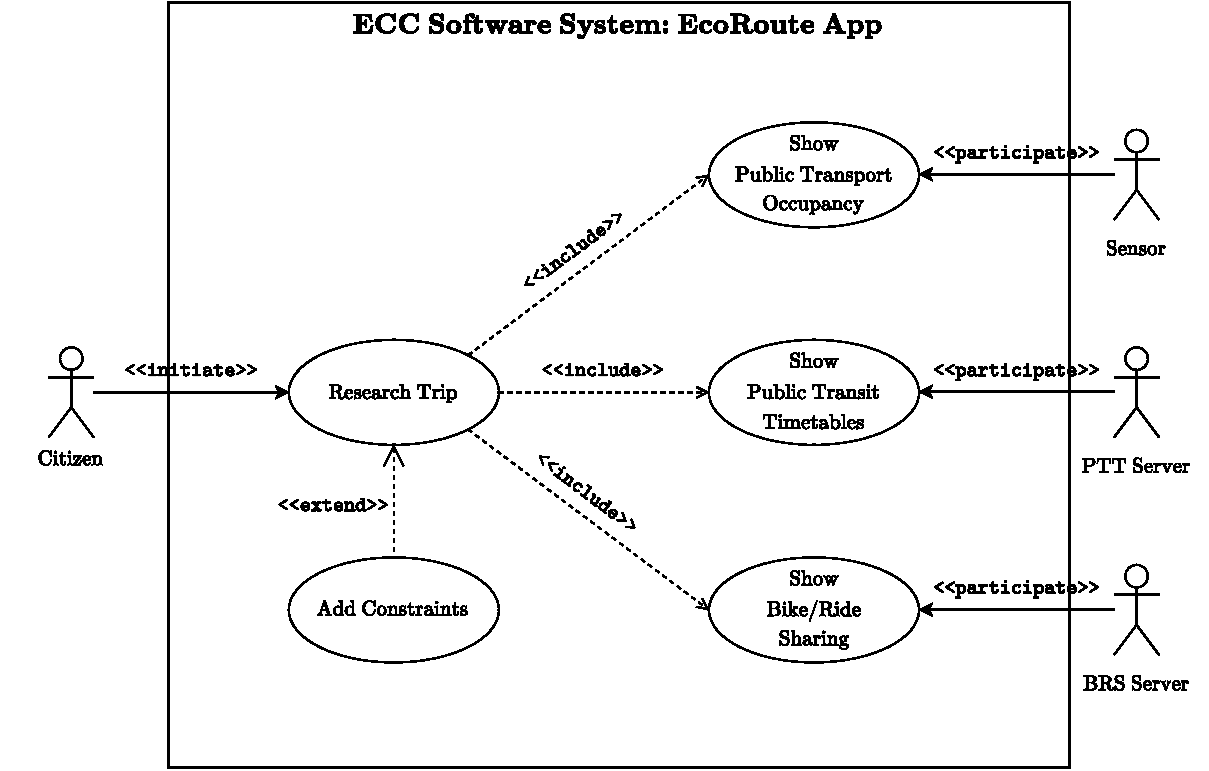
\includegraphics[width=\textwidth]{img/use-cases.pdf}
        \caption{Use case diagram for the EcoRoute App.}
        \label{fig: use case diagram}
    \end{figure}

    \noindent
    To view/download the Use Case Diagram in high quality, click or scan the QR code below:
    \begin{center}
        \qrcode{https://polimi365-my.sharepoint.com/:b:/g/personal/11010856_polimi_it/ERGPI0u-a-BOuDhhvbXgIuYB80fiMnHUGrw-sSqx9BaRbQ}
    \end{center}

    \noindent
    As we can see from the use case diagram (Figure~\ref{fig: use case diagram}), there are 5 use cases identified. On page~\pageref{Use Case - Research Trip}, in Table~\ref{Use Case - Research Trip}, we give an exhaustive explanation of the Research Trip use case. However, in the following list, we talk about the other use cases:
    \begin{itemize}
        \item \textbf{Show Public Transport Occupancy}. The Public Transport Occupancy is a crucial resource gathered by the EcoRoute (app) from the sensors deployed on the Public Transport and used to avoid bottlenecks at peak times. 
        
        We have included this use case in the Research Trip use case.

        \newpage

        \item \textbf{Show Public Transit Timetables}. The Public Transit Timetables are essential for finding the correct public transport route for the user. The app also uses them to find (and combine) the most environmentally friendly route. 
        
        We have included this use case in the Research Trip use case.


        \item \textbf{Show Bike/Ride Sharing}. Bike/Ride Sharing is mainly used to suggest more ecological means of transport to the user, such as bicycles. The app also uses it to combine with public transport. We have included this use case in the Research Trip use case.


        \item \textbf{Add Constraints}. The user can add constraints, but this choice is not required by the system (as the project problem says). So the user can decide if to impose some limitations or not. We have extended the Research Trip use case with this use case.
    \end{itemize}
    
    \begin{table}[!htp]
        \centering
        \begin{tabular}{@{} l p{23em} @{}}
            \toprule
            \multicolumn{2}{c}{Use Case: \textbf{Research Trip}} \\ 
            \midrule
            %%%
            Primary Actor 
            & 
            Citizen. \\ \\
            %%%
            Supporting Actor 
            & 
            ~~\llap{\textbullet}~~ Sensor;

            ~~\llap{\textbullet}~~ PTT Server (Public Transit Timetable);

            ~~\llap{\textbullet}~~ BRS Server (Bike-Ride-Sharing). \\ \\
            %%%
            Description 
            &
            A citizen, the application user, inserts the information about their trip. The information required is the origin and the destination. The constraints can be optional (Add Constraints use case extend Research Trip). 
            
            Once the user does the research (e.g., by clicking the \dquotes{research} button), three use cases extend the Research Trip: the Sensor, the PTT Server, and the BRS Server participate in the research made by the user, showing the different ecological choices. 
            
            The user sees the final result, but the app makes the low-level requests, calculations, and others. \\ \\
            %%%
            Data 
            &
            Origin, destination, (optional) constraints, environmentally friendly routes. \\ \\
            %%%
            Comments 
            &
            The citizen must enter the origin and destination within the urban area. \\
            \bottomrule
        \end{tabular}
        \caption{Detailed use case explanation - Research Trip.}
        \label{Use Case - Research Trip}
    \end{table}

    \newpage

    \subsection{Domain assumptions}

    The domain properties are descriptive assertions that are assumed to hold in the world (the part of the real world that is affected by the \dquotes{machine}, in our case EcoRoute). In this project, the domain assumptions are as follows:
    \begin{itemize}
        \item \emph{Sensors are correctly deployed on public transport means and can share occupancy rates with the ECC.}
        
        \item \emph{Public transit timetables are available and can be acquire in real-time from the ECC.}

        \item \emph{Services that offers bike and/or ride sharing can share their information with the ECC.}
        
        \item \emph{The Citizens stakeholder interacts with the software system provided by the ECC through a mobile application (called EcoRoute).}
        
        \item \emph{Citizens must have an internet connection to use the mobile application.}
    \end{itemize}

    \newpage

    \subsection{Requirements}
    
    \subsubsection{Functional requirements}

    The functional requirements describe the interactions between the system and its environment. Then our application provides the following requirements:
    \begin{itemize}
        \item The mobile application will allow users (citizens):
        \begin{itemize}
            \item To find an environmentally friendly route.

            \item To add any constraints.
            
            \item To view all or one of the Public Transport Occupancy, Public Transit Timetables, Bike/Ride Sharing information in the final result.
        \end{itemize}

        \item The system should guarantee that the environmentally friendly route computed is the most eco-friendly and give preference to combinations of different modes of transport.
    \end{itemize}

    \subsubsection{Non-functional requirements}

    The non-functional requirements specify or constrain characteristics of the system as a whole. Then our application provides the following requirements:
    \begin{itemize}
        \item The EcoRoute application must be available to all users (citizens) 24 hours a day, 7 days a week, including public holidays.
        

        \item Downtime during normal working hours should not exceed 1 minute, as this is when the application is most used by citizens.
        
        Holiday downtime should not exceed 5 minutes.

        
        \item The algorithm time to calculate the best environmentally friendly routes should not exceed 10 seconds.
    \end{itemize}

    \newpage

    \section{Design}

    \subsection{General description of the architecture}

    The architecture chosen for the EcoRoute project is Client-Server, but with the worker pooling (\href{https://www.nginx.com/}{NGINX web server}). The reason for this choice is discussed in section~\ref{subsection: Critical points and design decisions} on page~\pageref{subsection: Critical points and design decisions}.

    \hfill

    \begin{figure}[!htp]
        \centering
        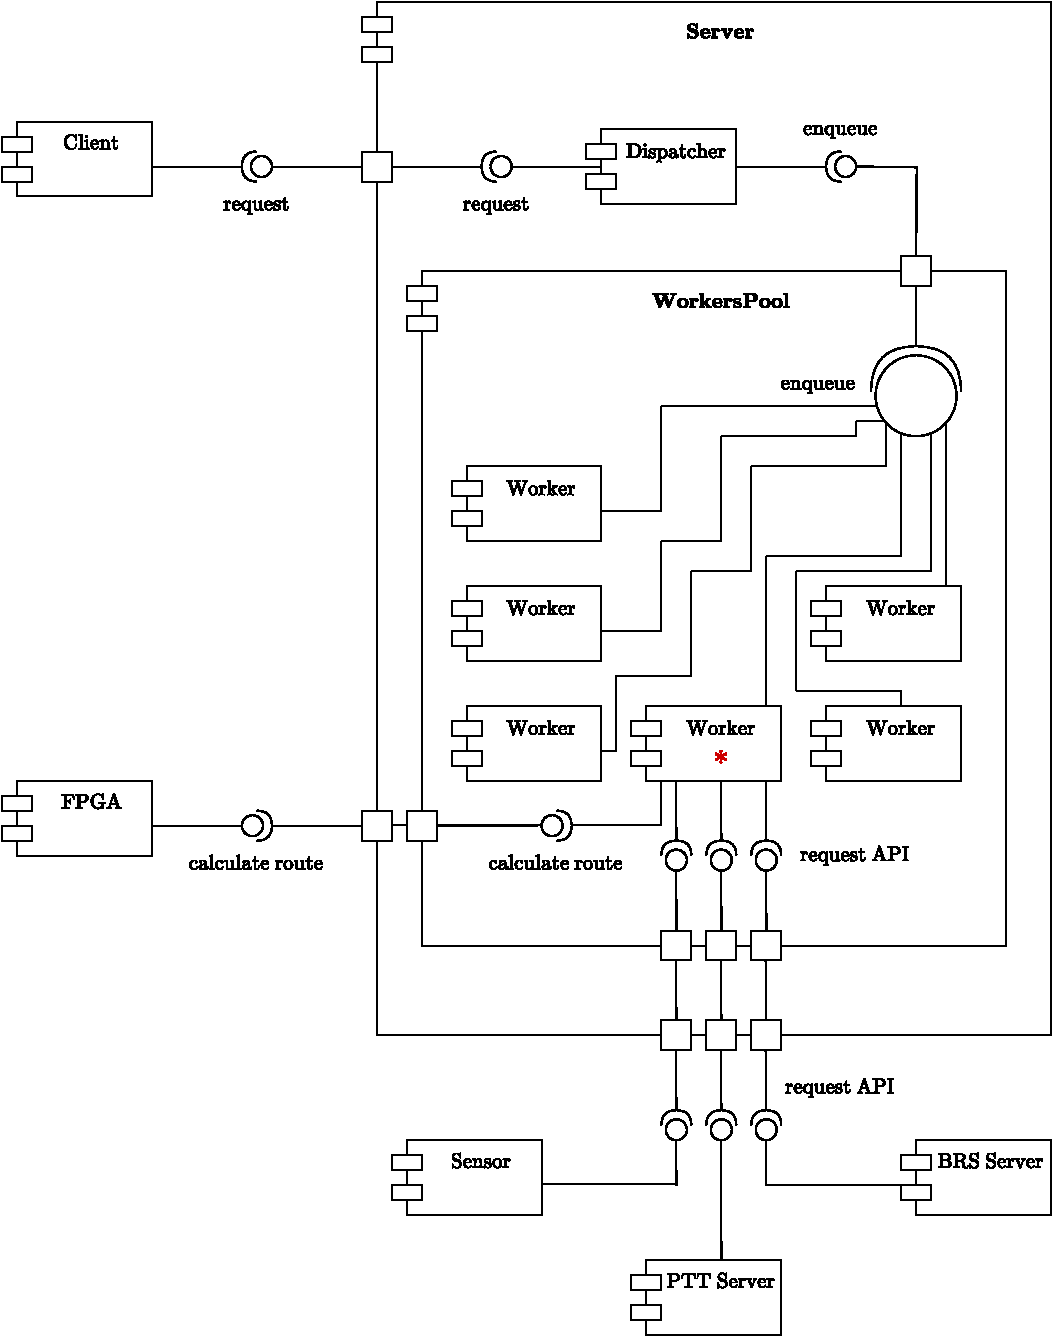
\includegraphics[width=\textwidth]{img/component-diagram.pdf}
        \caption{Component Diagram for the EcoRoute App.}
        \label{fig: component diagram}
    \end{figure}

    \hfill
    
    \newpage

    \noindent
    To view/download the Component Diagram in high quality, click or scan the QR code below:
    \begin{center}
        \qrcode{https://polimi365-my.sharepoint.com/:b:/g/personal/11010856_polimi_it/EecFf7fmu2FKp-33kGvRWRUB-9IOZYE1OLVhxTJCb7d91w}
    \end{center}

    \noindent
    Before we go into details, let us assume that sensors are deployed on public transport means and that they publish updated data on occupancy rates at each stop. The data are saved into a HPC database, such as \href{https://www.scylladb.com/}{ScyllaDB}. We have analyzed this assumption again in the section~\ref{subsection: Critical points and design decisions} on page~\pageref{subsection: Critical points and design decisions}.

    \highspace
    (\textcolor{Red3}{\textbf{*}}) It is also important to note that only one module (Worker) is connected to the Sensor, PTT Server and BRS Server. This is a design choice to avoid a less readable component diagram. We can imagine that each Worker is connected to Sensor, PTT Server and BRS Server.

    \highspace
    The following list examines each component of the component diagram (Figure~\ref{fig: component diagram}):
    \begin{itemize}
        \item \textbf{Client}. The module represents the application installed on the stakeholder's (citizen's) device. The aim of the module is to send requests to the server to calculate the route requested by the citizen.

        \item \textbf{Server}. The server module is the NGINX web server (worker pooling technology). It is installed on the server side of the application and can be considered as the core of the architecture. In fact, its aim is to manage the high traffic of requested and instantiated resources. It also aims to send asynchronous requests to the different servers to obtain data about the services requested by the client. Finally, it can request the calculation of the route by interrogating the FPGA module.

        \item \textbf{Dispatcher}. This is the module that takes the request from the client and instantiates the resource. It can enqueue a request into a worker queue if a resource is unavailable. To maintain high performance and optimize scalability, the dispatcher can also drop incoming requests if the worker queues are full (we sacrifice availability in this case). 

        \item \textbf{Workers and Workers Pool}. The worker pool is a container in which we can find 6 workers. Each worker can send (asynchronous) requests to the different servers to obtain the data necessary to calculate the best environmentally friendly routes. Finally, each worker can also delegate the calculation of the route to the FPGA module.
        
        Note that we follows the rule: one worker for each CPU core.\footnote{Source: \href{https://www.nginx.com/blog/inside-nginx-how-we-designed-for-performance-scale/}{Inside NGINX: How We Designed for Performance \& Scale}}

        \item \textbf{Sensor (ScyllaDB)}. It is the module that interacts with the database that contains the data of the transport lines. In order to have a high performance, we assume that the database is a \href{https://www.scylladb.com/product/technology/}{ScyllaDB} and this module can query this resource.

        \item \textbf{PTT Server}. It is the module that interacts with the Public Transit Timetable Server. It can take the data from this resource. This module is an interface that allows to have a great generalization in order to implement as many services as we want. For example, we can easily implement ATM (Milan) or ATV (Verona).
        
        \item \textbf{BRS Server}. As a PTT server logic, this module can interact with the Bike/Ride Sharing server. This module is also a perfect generalization as a PTT server.

        \item \textbf{FPGA}. This is the module that interfaces with the FPGA hardware. This hardware may be physically located in the server room or in a service such as \href{https://aws.amazon.com/ec2/instance-types/f1/}{Amazon F1 EC2}.
    \end{itemize}    

    \newpage

    \subsection{Sequence diagrams}

    \begin{figure}[!htp]
        \centering
        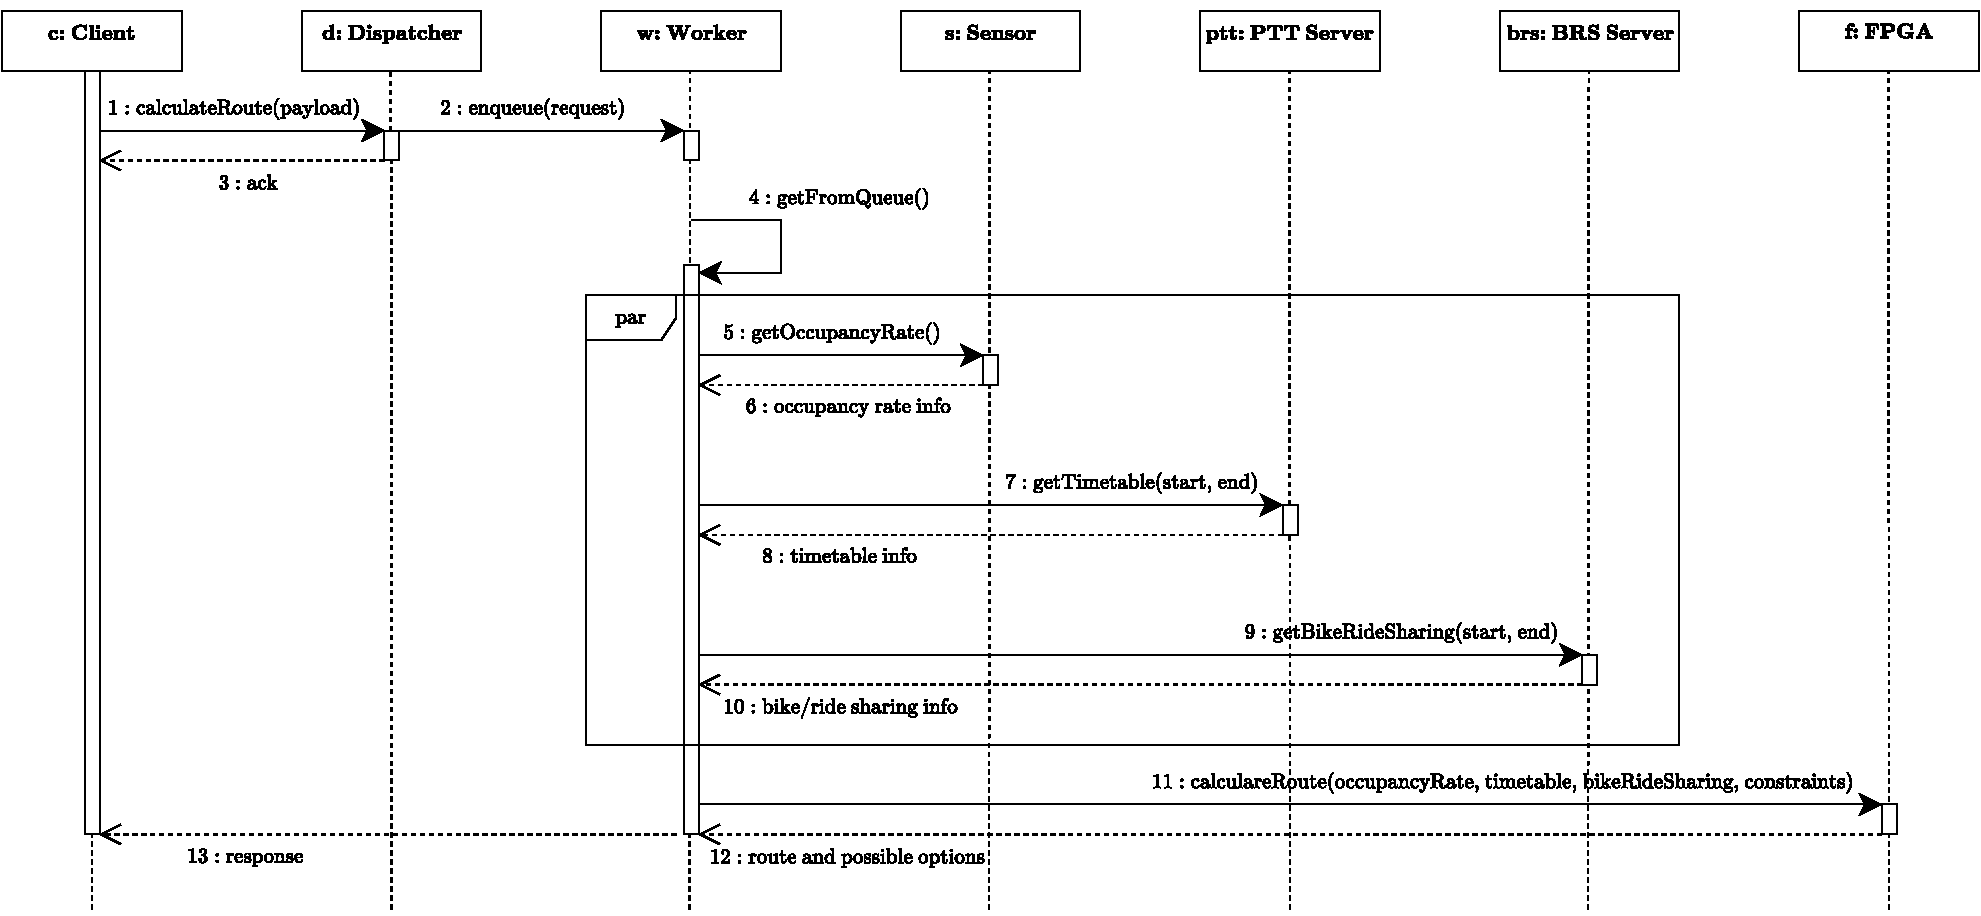
\includegraphics[width=\textwidth]{img/sequence-diagram-1.pdf}
    \end{figure}

    \begin{figure}[!htp]
        \centering
        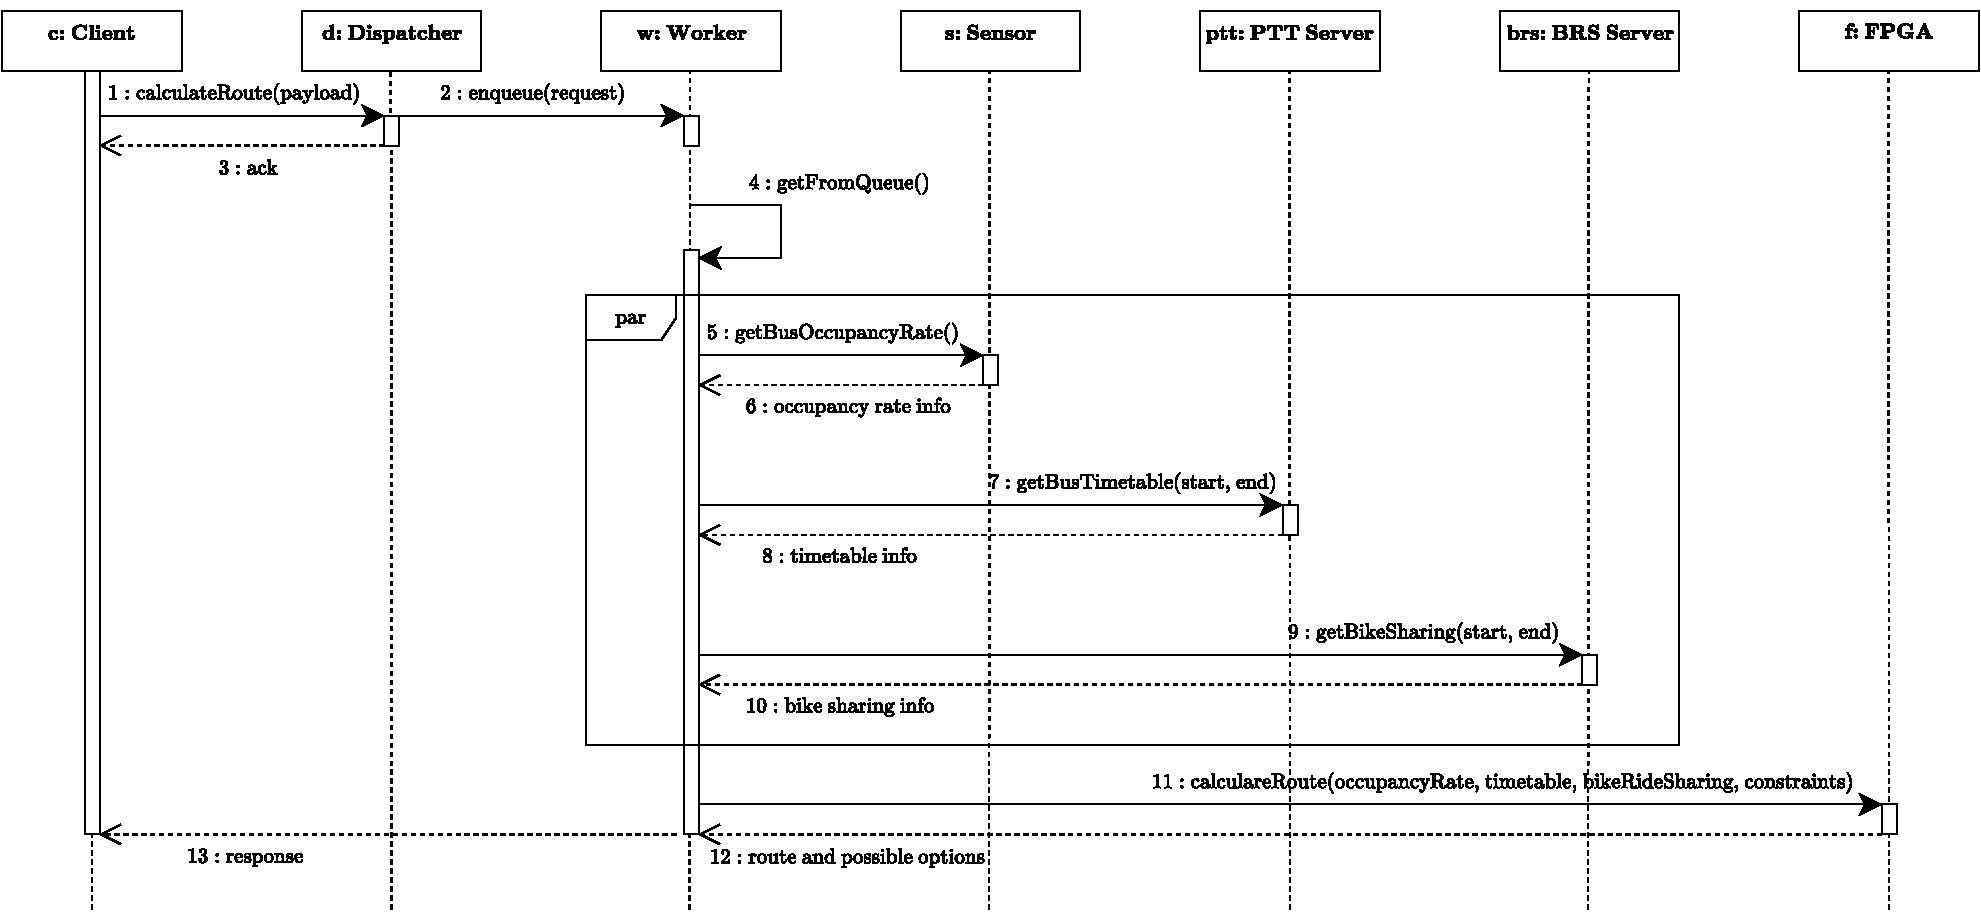
\includegraphics[width=\textwidth]{img/sequence-diagram-2.pdf}
    \end{figure}

    \begin{figure}[!htp]
        \centering
        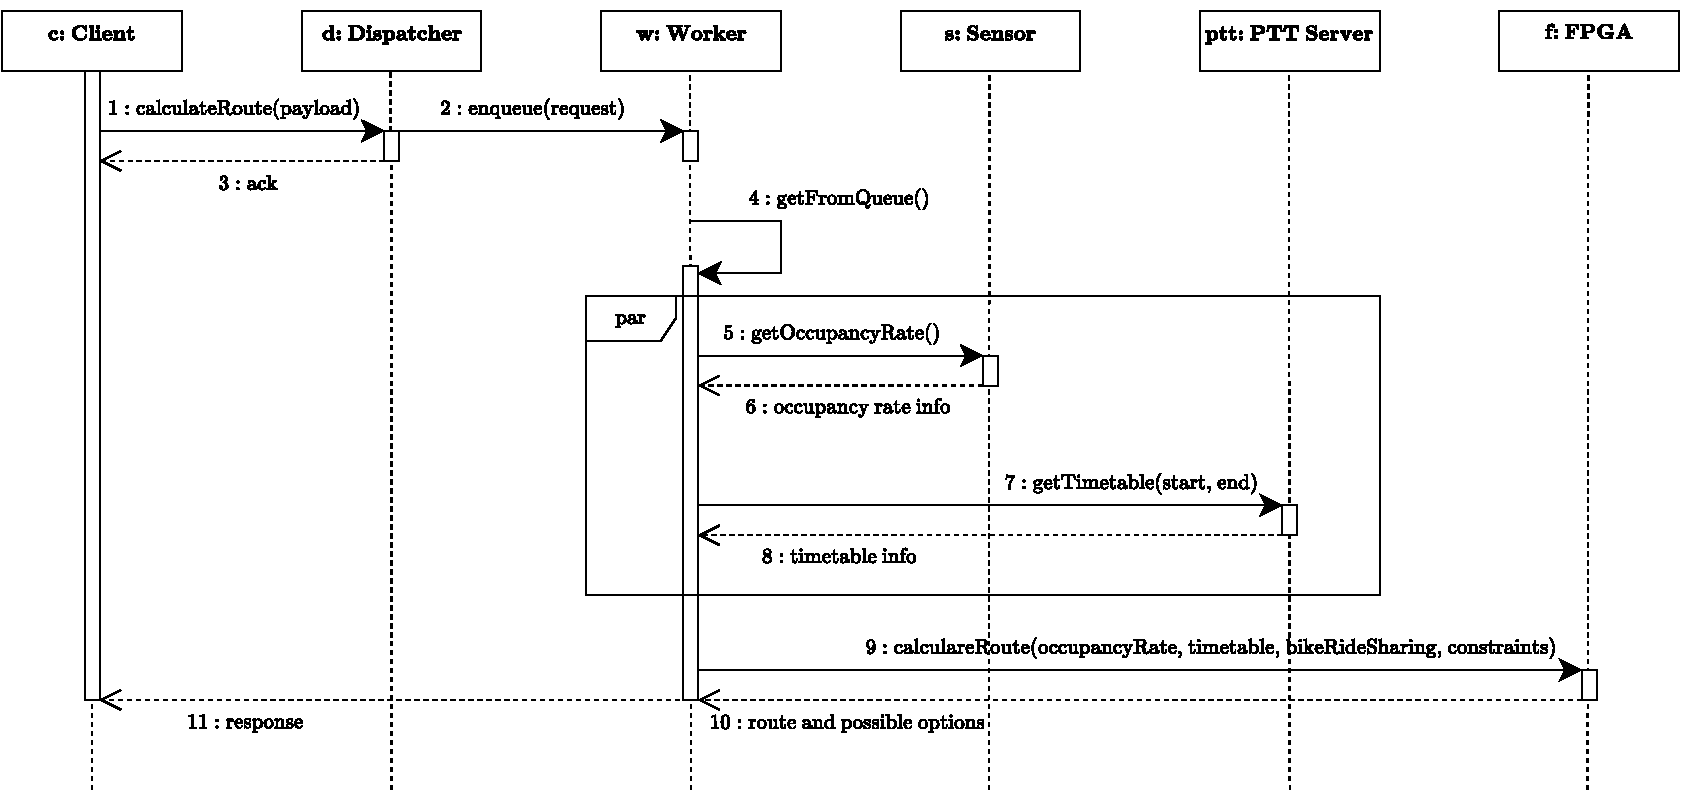
\includegraphics[width=\textwidth]{img/sequence-diagram-3.pdf}
    \end{figure}

    \begin{figure}[!htp]
        \centering
        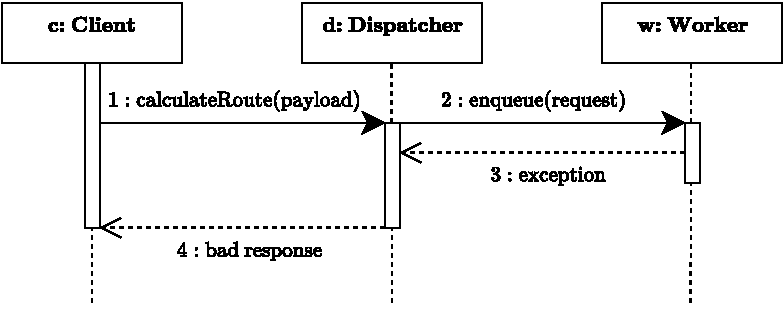
\includegraphics[width=\textwidth]{img/sequence-diagram-4.pdf}
    \end{figure}

    

    % IDEA:
    % 1. Client make a simple request with no constraints.
    % 2. Client make a request with a constraint: he wants to use bike sharing and bus service.
    % 3. Client make a request excluding a service, such as bike and car sharing. We give him the option but under the field "Do you search an other service?"
    % 4. Extreme case: the each worker queue is full! Request denied.

    \newpage

    \subsection{Critical points and design decisions}\label{subsection: Critical points and design decisions}
\end{document}